Dynamic Data Management currently manages a pool of approximately 20 PB across several Tier 2 and Tier 1 sites. Datasets which are considered deprecated are deleted, while those which are very popular are replicated at multiple sites. A good measure of the performance of this algorithm is the number of accesses per replica. If this number is very small, then the dataset is not being replicated according to its popularity. On the other hand, if it is very small for many datasets, then we are maintaining too many copies of unused datasets. To make popularity plots as shown in Figure~\ref{fig:usage}, four attributes are computed for each dataset: number of accesses, size on disk, number of files, and average number of replicas.

\begin{figure}[htbp]
    \centering
    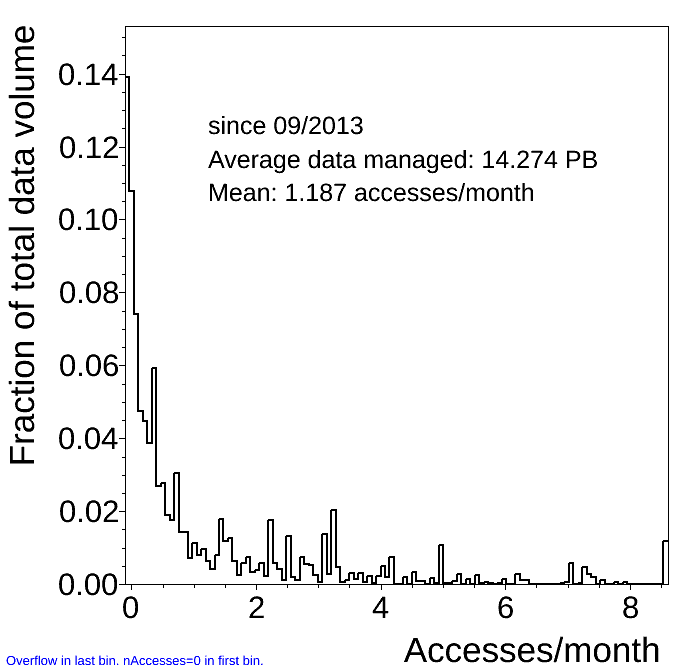
\includegraphics[width=0.45\textwidth]{plots/DatasetSummaryAll_nSitesAverage.png}
    \caption{Dataset usage plot for the time interval $[09/2013,\text{present}]$}
    \label{fig:usage}
\end{figure}

% In order to identify 
% the very few, rare events that are clear signatures of new physics in our detector, we must optimally use the available 
% computing resources. The computing challenge will become harder with time, as the amount of collected data will increase 
% substantially in the years to come. The schedule at present foresees two major data taking phases - Run-II and Run-III - 
% which have the following characteristics (Run-I is also shown for comparison):

% \begin{itemize}
% 	\item Run-I: 2010-2012, nominal collision energy 7(8) TeV, accumulated data \\ 50 PB (5(20) \fbinv); 
% 	\item Run-II: 2015-2017, nominal collision energy 13 TeV, accumulated data \\ 200 PB ($\sim$ 100 \fbinv); 
%	\item Run-III: 2019-2021, nominal collision energy 14 TeV, accumulated data \\ 400 PB ($\sim$ 300 \fbinv). 
% \end{itemize}
% The numbers are staggering and while computing resources will grow and algorithmic adjustments will be made as well, it is 
% obvious that an optimization of the present system is going to have a major impact on this endeavor.

% CMS is now proposing to make best use of our computing resources by employing a novel way of managing the data distribution, based on a dynamic system that will be able to optimize the performance using a number of different system metrics.
% The plan is to treat all CMS computing sites as a network of massive caches. The optimization of the CMS data distribution in these caches is a challenging task because the system contains order of 50 geographically separated computing centers of quite different properties, and the computing tasks to be performed on them cover a wide parameter space in terms of their computing requirements. Considering the complexity of the optimization problem with perfectly working components and further including component failures into the task it is clear that there is no analytic solution and machine learning algorithms seem a great candidate to achieve a reliable and - once properly trained - low maintenance solution.

% While this is a long term project that is involving the large computing community of CMS, the MIT HEP computing group has been pioneering techniques to perform 
% automated data management at our local facilities, and here we document the core functionalities of the system that we designed, 
% translated into software, tested and put into production.
